The self-protection suite consists of a pod located under the left-hand wing and a cockpit unit connected by existing wiring. The pod is able to intelligently dispense two (2) loads of chaffs and flares simultaneously, and can dispense forwards, downwards and sideways. Furthermore, the pod contains a missile warning system (MWS), which provides the pilot with both visible and audible warnings when threats occur.

The self-protection suite is able to automatically detect threats, and dispense payloads in advance without pilot interaction. The pilot may choose other modes of operation, offering varying degrees of control.
\begin{figure}[h]
	\centering
	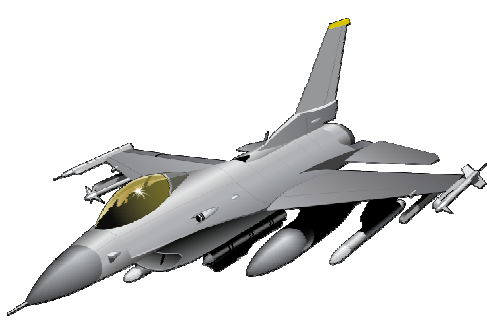
\includegraphics[scale=0.5]{./images/F16.PNG}\\
	\caption{F-16 combat aircraft}
\end{figure}
